% ============================================================================
% Research Proposal — Clean & Compact Academic Format
% ============================================================================
\documentclass[12pt,a4paper]{article}

% --- Packages ---------------------------------------------------------------
\usepackage[utf8]{inputenc}
\usepackage[T1]{fontenc}
\usepackage{lmodern}
\usepackage[margin=1in]{geometry}
\usepackage{setspace}
\usepackage{titlesec}
\usepackage{enumitem}
\usepackage{booktabs}
\usepackage{tabularx}
\usepackage{graphicx}
\usepackage{amsmath,amssymb}
\usepackage{hyperref}
\usepackage{url}
\usepackage{cite}
\usepackage{fancyhdr}
\usepackage{float}
\usepackage{caption}
\usepackage{tikz}
\usetikzlibrary{shapes.geometric, arrows.meta, positioning, fit, backgrounds}

% --- Spacing ----------------------------------------------------------------
\onehalfspacing

% --- Page Style -------------------------------------------------------------
\pagestyle{fancy}
\fancyhf{}
\setlength{\headheight}{15pt}
\renewcommand{\headrulewidth}{0.4pt}
\fancyhead[L]{\small\textit{Research Proposal}}
\fancyhead[R]{\small\textit{Smart Grid Cybersecurity}}
\fancyfoot[C]{\thepage}

% --- Section Formatting -----------------------------------------------------
\titleformat{\section}{\large\bfseries}{\thesection.}{0.5em}{}
\titleformat{\subsection}{\normalsize\bfseries}{\thesubsection}{0.5em}{}
\titleformat{\subsubsection}{\normalsize\itshape}{\thesubsubsection}{0.5em}{}

% --- Hyperref ---------------------------------------------------------------
\hypersetup{
  colorlinks=true,
  linkcolor=black,
  citecolor=black,
  urlcolor=blue!60!black
}

% ============================================================================
\begin{document}

% --- Title Page -------------------------------------------------------------
\begin{titlepage}
\centering
\vspace*{1.5cm}

{\Large\textbf{RESEARCH PROPOSAL}}

\vspace{0.8cm}

\rule{\textwidth}{1pt}
\vspace{0.4cm}

{\LARGE\bfseries Cryptographic Latency Exploitation and Wire-Speed Defense in IEC 61850 Smart Grid Substation Automation Systems}

\vspace{0.4cm}
\rule{\textwidth}{1pt}

\vspace{2cm}

{\large
\textbf{Research Guide}\\[0.2cm]
{\Large\textbf{Dr.~Sapna~V.~M.}}\\[0.15cm]
PES University
}

\vfill

{\large \today}

\end{titlepage}

% --- Table of Contents ------------------------------------------------------
\newpage
\tableofcontents
\newpage

% ============================================================================
\section{Title of the Research}
% ============================================================================

\textbf{``Cryptographic Latency Exploitation and Wire-Speed Defense in IEC~61850 Smart Grid Substation Automation Systems''}

\vspace{0.5cm}

\noindent\textbf{Domain:} Cybersecurity of Critical Infrastructure / Smart Grid Security / Industrial Control Systems (ICS)

\noindent\textbf{Sub-Domain:} Protocol-Level Vulnerability Analysis, Real-Time Cyber-Physical System Defense, Kernel-Level Packet Filtering (eBPF/XDP)

\noindent\textbf{Research Guide:} Dr.~Sapna~V.~M., PES University

% ============================================================================
\section{Introduction}
% ============================================================================

The electrical power grid is undergoing rapid modernization driven by the integration of digital communication technologies into substation automation systems. Central to this transformation is the \textbf{IEC~61850} international standard, which defines communication protocols for Intelligent Electronic Devices (IEDs) --- the networked protection relays, circuit breaker controllers, and metering units that form the backbone of modern substations~\cite{iec61850}.

Among the protocols defined by IEC~61850, the \textbf{GOOSE (Generic Object Oriented Substation Events)} protocol is safety-critical. GOOSE enables peer-to-peer, multicast communication over raw Ethernet (Layer~2, EtherType \texttt{0x88B8}) for time-critical protection signaling. When a fault is detected on a transmission line --- such as a short circuit on a 220~kV feeder --- a protection relay must transmit a trip command to the corresponding circuit breaker. This trip command \textbf{must be processed within 3~ms} as mandated by \textbf{IEC~61850-5} for Type 1A (Performance Class P2/P3) high-voltage trip applications to prevent physical destruction of power equipment, including transformers (replacement cost: \$2--10M USD; lead time: 12--18 months), generators, and switchgear~\cite{sel_relay, iec61850}.

The original GOOSE protocol was designed for maximum speed and provides \textbf{no native authentication or encryption}. Any device on the substation LAN can inject, replay, or modify GOOSE messages. This fundamental vulnerability was exploited in real-world attacks, most notably by the \textbf{Industroyer/CrashOverride} malware during the 2016 Ukraine power grid attack, which included a dedicated IEC~61850 protocol module for automated circuit breaker manipulation~\cite{industroyer, ukraine2015}.

To address this vulnerability, the \textbf{IEC~62351-6} standard introduces cryptographic authentication for GOOSE messages using HMAC-SHA256 or RSA-2048 digital signatures~\cite{iec62351}. However, this security measure introduces a critical conflict: \textbf{cryptographic verification consumes significant CPU time on resource-constrained IED hardware}, potentially threatening the real-time safety guarantees that the protocol was designed to provide.

This research investigates the hypothesis that the introduction of cryptographic security in smart grid communications creates an unexplored security-safety trade-off that can be exploited via targeted latency attacks.

% ============================================================================
\section{Problem Statement}
% ============================================================================

The deployment of IEC~62351 cryptographic authentication on IEC~61850 GOOSE communications introduces a fundamental \textbf{security--safety paradox}: the mechanism designed to protect the grid may itself become the vector that compromises real-time responsiveness.

On resource-constrained IED processors (ARM Cortex-R/M class, 200--600~MHz typical of legacy protection relays), cryptographic signature verification operations introduce non-trivial processing overhead. Table~\ref{tab:crypto_latency} outlines representative latency estimates reported in literature~\cite{strobel2016}, which will be empirically measured and validated on our testbed setup.

\begin{table}[H]
\centering
\caption{Representative Cryptographic Verification Latency on IED-Class Hardware}
\label{tab:crypto_latency}
\vspace{0.2cm}
\begin{tabularx}{\textwidth}{X c c}
\toprule
\textbf{Cryptographic Operation} & \textbf{Latency (ms)}~\cite{strobel2016} & \textbf{Margin vs.\ 3~ms Deadline} \\
\midrule
GOOSE Parse (ASN.1 BER-TLV) & 0.05 -- 0.15 & Bounded ($< 0.15$~ms) \\
HMAC-SHA256 Verification & 0.3 -- 0.8 & 2.0 -- 2.7~ms \\
RSA-2048 Signature Verification & 1.5 -- 5.0 & $-$2.0 to 1.5~ms (Deadline Risk) \\
ECDSA-P256 Signature Verification & 2.0 -- 8.0 & $-$5.0 to 1.0~ms (High Violation Risk) \\
\bottomrule
\end{tabularx}
\end{table}

An attacker with Layer~2 access to the substation network can exploit this computational cost by flooding the IED with structurally valid GOOSE frames carrying \textbf{invalid cryptographic signatures}. Each frame forces the IED's CPU to perform full signature verification before determining that the frame is invalid. Under sustained flood conditions, the verification queue saturates, and legitimate protection trip messages are delayed beyond the 3~ms safety deadline --- resulting in circuit breaker failure, equipment destruction, and potential cascading grid failures.

To the best of our knowledge, existing literature has not comprehensively investigated this \textbf{Crypto-Induced Latency Denial of Service (CIL-DoS)} vulnerability class. Prior research on GOOSE security predominantly focuses on spoofing, replay, and man-in-the-middle attacks, but does not deeply evaluate the systemic latency impact of cryptographic verification under high-rate adversarial traffic.

Furthermore, traditional firewalls and user-space Intrusion Detection Systems (IDS) operate at higher layers of the network stack, introducing additional packet processing overhead. A suitable defense requires \textbf{wire-speed filtering} to drop malicious packets before they consume CPU-intensive cryptographic verification queues on the target device.

% ============================================================================
\section{Threat Model}
% ============================================================================

To formally evaluate the security posture of IEC~61850/IEC~62351 environments, we define explicit threat boundaries, attacker assumptions, protected assets, and adversarial goals.

\subsection{Attacker Assumptions}
\begin{enumerate}[noitemsep]
  \item \textbf{Layer-2 Access:} The attacker has gained access to the internal substation local area network (LAN) via a compromised maintenance laptop, rogue wireless access point, or compromised IT/OT gateway interface.
  \item \textbf{No Cryptographic Key Compromise:} The attacker does \emph{not} possess the private key or shared HMAC secret key used by legitimate IEDs for signing GOOSE frames.
  \item \textbf{No Firmware Compromise:} The attacker cannot modify the target IED's firmware or internal operating system logic directly.
  \item \textbf{No Physical Device Access:} The attacker does not possess physical access to tamper with the relay hardware, wiring, or trip coils directly.
\end{enumerate}

\subsection{Protected Assets}
\begin{itemize}[noitemsep]
  \item \textbf{Intelligent Electronic Devices (IEDs):} Digital protection relays executing real-time automation and safety logic.
  \item \textbf{Circuit Breakers:} High-voltage physical switching equipment responsible for isolating electrical faults.
  \item \textbf{Substation Safety Margins:} The hard $\le 3$~ms real-time deadline mandated for GOOSE trip execution by IEC~61850-5 (Type 1A Class P2/P3)~\cite{iec61850}.
\end{itemize}

\subsection{Adversarial Goals}
\begin{itemize}[noitemsep]
  \item \textbf{Primary Goal:} Induce protection deadline misses ($\ge 3$~ms delay) during physical fault events to cause physical damage or arc flashes.
  \item \textbf{Secondary Goal:} Exhaust CPU resources on target protection relays without triggering conventional rate-based alarm thresholds.
\end{itemize}

% ============================================================================
\section{Research Questions, Hypotheses, and Expected Contributions}
% ============================================================================

This research addresses four explicit research questions alongside testable hypotheses:

\begin{enumerate}[leftmargin=1.5cm]
  \item[\textbf{RQ1.}] \emph{Can cryptographic verification latency alone violate IEC~61850 real-time timing guarantees under adversarial flood conditions?}
  \begin{itemize}[noitemsep, label=$\rightarrow$]
    \item \textbf{Hypothesis H1:} Cryptographic signature verification under sustained adversarial traffic floods will cause protection message processing latency to exceed the 3~ms safety-critical deadline on resource-constrained IEDs.
  \end{itemize}

  \item[\textbf{RQ2.}] \emph{Under what specific traffic rates, frame structures, and cryptographic algorithms does the CIL-DoS attack state emerge?}
  \begin{itemize}[noitemsep, label=$\rightarrow$]
    \item \textbf{Hypothesis H2:} We hypothesize that queue saturation begins when the packet arrival rate approaches or exceeds the effective cryptographic verification service rate, which will be modeled using queueing theory and validated experimentally.
  \end{itemize}

  \item[\textbf{RQ3.}] \emph{Can an eBPF/XDP driver-level packet filter restore deterministic, bounded timing for legitimate trip commands under active CIL-DoS floods?}
  \begin{itemize}[noitemsep, label=$\rightarrow$]
    \item \textbf{Hypothesis H3:} An inline eBPF/XDP pre-filter operating at the NIC driver level can drop $>99\%$ of invalid signature packets before queue insertion, restoring trip latency to $\le 3$~ms.
  \end{itemize}

  \item[\textbf{RQ4.}] \emph{What is the performance trade-off between kernel-space (XDP) inline filtering and user-space stateful anomaly detection in smart grid environments?}
  \begin{itemize}[noitemsep, label=$\rightarrow$]
    \item \textbf{Hypothesis H4:} Driver-level XDP filtering will achieve sub-microsecond processing overhead per frame, outperforming user-space IDS solutions by at least two orders of magnitude in terms of throughput capacity.
  \end{itemize}
\end{enumerate}

\subsection{Expected Scientific Contributions (Delineation of Proposed Work)}

To maintain a clear boundary between established background state-of-the-art and our original research, Table~\ref{tab:contributions_delineation} explicitly delineates our proposed scientific contributions.

\begin{table}[H]
\centering
\caption{Delineation between Established Literature and Proposed Contributions}
\label{tab:contributions_delineation}
\vspace{0.2cm}
\begin{tabularx}{\textwidth}{p{4.5cm} X}
\toprule
\textbf{Category} & \textbf{Specific Elements} \\
\midrule
\textbf{Established Background} & IEC 61850/62351 standards~\cite{iec61850, iec62351}, 3~ms timing deadline~\cite{iec61850}, prior grid attacks (Industroyer, BlackEnergy)~\cite{industroyer, ukraine2015}, baseline eBPF/XDP primitives~\cite{ebpf_iot}. \\
\midrule
\textbf{Proposed Contribution C1} & \textbf{Formal Characterization of CIL-DoS:} First systematic taxonomy and formal mathematical model of Crypto-Induced Latency DoS attacks. \\
\textbf{Proposed Contribution C2} & \textbf{Queueing-Theoretic Saturation Model:} Queueing model formulating verification queue buildup and deadline violation boundaries. \\
\textbf{Proposed Contribution C3} & \textbf{Open-Source Research Toolkit:} Zero-dependency Python suite for real-time IEC~61850 GOOSE/DNP3 frame synthesis and analysis. \\
\textbf{Proposed Contribution C4} & \textbf{Wire-Speed Mitigation Framework:} Driver-level eBPF/XDP filter enforcing stNum/sqNum monotonicity and rate validation at line-rate. \\
\bottomrule
\end{tabularx}
\end{table}

% ============================================================================
\section{Research Objectives}
% ============================================================================

The primary objectives of this research are:

\begin{enumerate}[leftmargin=2cm]
  \item[\textbf{RO1.}] To \textbf{formally analyze} the Crypto-Induced Latency Denial of Service (CIL-DoS) vulnerability in IEC~62351-protected IEC~61850 GOOSE communications.

  \item[\textbf{RO2.}] To \textbf{develop protocol tooling} --- including a zero-dependency IEC~61850 GOOSE protocol parser/builder and a DNP3 protocol parser --- enabling reproducible security research.

  \item[\textbf{RO3.}] To \textbf{design attack tools} that simulate the CIL-DoS vulnerability, including GOOSE injection, replay, and signature flood capabilities.

  \item[\textbf{RO4.}] To \textbf{design and implement a wire-speed defense mechanism} using Linux eBPF/XDP (eXpress Data Path) technology to filter invalid packets at the NIC driver level.

  \item[\textbf{RO5.}] To \textbf{develop a stateful GOOSE Intrusion Detection System (IDS)} with protocol-aware anomaly detection and MITRE ATT\&CK for ICS mapping.

  \item[\textbf{RO6.}] To \textbf{rigorously evaluate defense effectiveness} across quantitative performance metrics including throughput, CPU utilization, queue occupancy, and deadline miss ratios.
\end{enumerate}

% ============================================================================
\section{Scope and Limitations of the Research}
% ============================================================================

\subsection{In Scope}

\begin{itemize}[noitemsep]
  \item Vulnerability analysis of IEC~61850 GOOSE and IEC~62351-6 authentication extensions
  \item Development of python-based protocol parser/builder libraries
  \item Implementation of GOOSE injection, replay, and CIL-DoS attack simulation scripts
  \item eBPF/XDP-based inline packet filtering program
  \item Stateful GOOSE intrusion detection logic
  \item Latency benchmarking of cryptographic operations on representative hardware
\end{itemize}

\subsection{Out of Scope}

\begin{itemize}[noitemsep]
  \item Exploitation of proprietary vendor firmware bugs or memory corruption vulnerabilities
  \item Experiments on live, operational utility grid infrastructure
  \item Hardware side-channel analysis
  \item MMS (Manufacturing Message Specification) protocol security analysis
\end{itemize}

\subsection{Limitations of the Study}

To maintain research transparency, we explicitly define the practical boundaries of this work:
\begin{enumerate}[noitemsep]
  \item \textbf{Testbed Environment:} All evaluations are conducted in controlled laboratory emulation testbeds. Real-world utility networks introduce hardware-specific variations.
  \item \textbf{Hardware Variations:} Performance metrics (such as exact XDP drop latency and CPU utilization) depend on specific Network Interface Cards (NICs) and CPU architectures.
  \item \textbf{Protocol Focus:} This study focuses specifically on Layer-2 GOOSE and IEC~62351-6 authentication rather than the entire multi-protocol suite of IEC~61850 (e.g., MMS or SV).
\end{enumerate}

% ============================================================================
\section{Literature Review}
% ============================================================================

\subsection{IEC~61850 and Substation Automation}

The IEC~61850 standard defines the communication architecture for substation automation systems. It specifies three primary communication protocols: GOOSE for fast event-based signaling, Sampled Values (SV) for current/voltage measurement streaming, and MMS for supervisory control~\cite{iec61850}. GOOSE operates directly over Ethernet at Layer~2, bypassing the TCP/IP stack to minimize processing overhead.

\subsection{Cyberattacks on Power Grid Infrastructure}

Substation automation security received heightened attention following confirmed cyberattacks on the Ukrainian power grid:
\begin{itemize}[noitemsep]
  \item \textbf{December 2015 (BlackEnergy):} Attackers compromised SCADA workstations to manually disconnect substations, impacting 230,000 customers~\cite{ukraine2015}.
  \item \textbf{December 2016 (Industroyer):} Automated attack framework featuring protocol payloads for IEC~60870-5-104, IEC~61850, and OPC DA to open circuit breakers directly~\cite{industroyer}.
\end{itemize}

In April 2026, ABB issued security advisory AV26-346 for \textbf{CVE-2025-3756}, highlighting a Denial of Service vulnerability in their IEC~61850 communication stack (CVSS 7.1)~\cite{cve2025}.

\subsection{IEC~62351 Implementation and eBPF Research}

Recent peer-reviewed studies have examined the computational trade-offs of IEC~62351 security extensions and programmable data planes in industrial control networks. Strobel et al. (2016) analyzed replay and time synchronization weaknesses in IEC~62351 implementations~\cite{strobel2016}. Hong et al. (2014) evaluated integrated anomaly detection architectures for substation communication channels~\cite{hong2014}.

In the domain of kernel-level filtering for critical infrastructure, Hoiland-Jorgensen et al. (2018) established the performance foundations of the eXpress Data Path (XDP) architecture~\cite{ebpf_iot}. Palumbo et al. (2024) demonstrated eBPF-based runtime security monitoring tailored for Industrial IoT protocols such as Modbus TCP~\cite{ebpf_modbus}.

\noindent\textbf{Research Gap:} To the best of our knowledge, existing literature has not comprehensively investigated the trade-off between cryptographic verification computation time and hard real-time safety constraints under high-velocity traffic conditions.

% ============================================================================
\section{Proposed Methodology and Comprehensive Evaluation Plan}
% ============================================================================

\subsection{Phase-Wise Methodology}
The project will be executed across protocol analysis, attack simulation, XDP kernel filter development, user-space IDS construction, and rigorous benchmarking.

\subsection{Evaluation Metrics and Desired Performance Objectives}
To rigorously evaluate hypotheses H1--H4 and answer RQs 1--4, explicit quantitative metrics and target performance objectives are defined in Table~\ref{tab:evaluation_metrics}.

\begin{table}[H]
\centering
\caption{Quantitative Evaluation Metrics and Target Performance Objectives}
\label{tab:evaluation_metrics}
\vspace{0.2cm}
\begin{tabularx}{\textwidth}{p{4.2cm} p{4.5cm} X}
\toprule
\textbf{Metric Category} & \textbf{Specific Metric (Unit)} & \textbf{Target Performance Objective} \\
\midrule
\textbf{Network Performance} & Attack Throughput (pps), Packet Loss (\%) & Line-rate handling ($>50\text{k pps}$) \\
\textbf{System Resources} & Target CPU Utilization (\%), Queue Depth & CPU utilization $< 30\%$ under attack \\
\textbf{Real-Time Impact} & End-to-End Trip Latency (ms), Miss Ratio & \textbf{Trip Latency $\le 3$~ms} ($0\%$ miss target) \\
\textbf{Defense Efficiency} & XDP Processing Latency ($\mu$s), Drop Rate & \textbf{XDP Latency $< 1$~$\mu$s}, Filter Drop $>99\%$ \\
\textbf{Detection Accuracy} & Accuracy (\%), FPR (\%), FNR (\%) & Accuracy $>99\%$, \textbf{False Positive Rate $<0.1\%$} \\
\bottomrule
\end{tabularx}
\end{table}

% ============================================================================
\section{Proposed System Architecture}
% ============================================================================

Figure~\ref{fig:layered_arch} presents the visual block diagram architecture of the GridPulse framework, detailing the modular pipeline across Network, Attack, Kernel, and User space layers.

\begin{figure}[H]
\centering
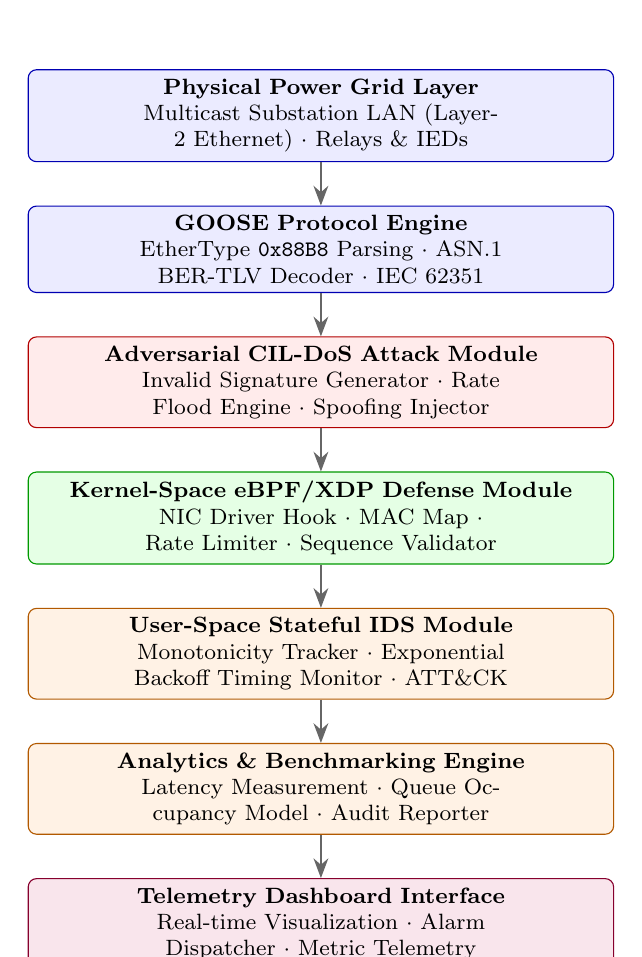
\begin{tikzpicture}[
  node distance=0.55cm and 0.8cm,
  block/.style={rectangle, draw=blue!70!black, fill=blue!8, text width=7.2cm, minimum height=0.95cm, rounded corners=3pt, font=\footnotesize, align=center},
  attack/.style={rectangle, draw=red!70!black, fill=red!8, text width=7.2cm, minimum height=0.95cm, rounded corners=3pt, font=\footnotesize, align=center},
  kernel/.style={rectangle, draw=green!60!black, fill=green!10, text width=7.2cm, minimum height=0.95cm, rounded corners=3pt, font=\footnotesize, align=center},
  user/.style={rectangle, draw=orange!70!black, fill=orange!10, text width=7.2cm, minimum height=0.95cm, rounded corners=3pt, font=\footnotesize, align=center},
  arrow/.style={-{Stealth[length=2.5mm]}, thick, color=gray!80!black}
]

  % System Components Nodes
  \node[block] (n1) {\textbf{Physical Power Grid Layer}\\Multicast Substation LAN (Layer-2 Ethernet) $\cdot$ Relays \& IEDs};
  \node[block, below=of n1] (n2) {\textbf{GOOSE Protocol Engine}\\EtherType \texttt{0x88B8} Parsing $\cdot$ ASN.1 BER-TLV Decoder $\cdot$ IEC 62351};
  \node[attack, below=of n2] (n3) {\textbf{Adversarial CIL-DoS Attack Module}\\Invalid Signature Generator $\cdot$ Rate Flood Engine $\cdot$ Spoofing Injector};
  \node[kernel, below=of n3] (n4) {\textbf{Kernel-Space eBPF/XDP Defense Module}\\NIC Driver Hook $\cdot$ MAC Map $\cdot$ Rate Limiter $\cdot$ Sequence Validator};
  \node[user, below=of n4] (n5) {\textbf{User-Space Stateful IDS Module}\\Monotonicity Tracker $\cdot$ Exponential Backoff Timing Monitor $\cdot$ ATT\&CK};
  \node[user, below=of n5] (n6) {\textbf{Analytics \& Benchmarking Engine}\\Latency Measurement $\cdot$ Queue Occupancy Model $\cdot$ Audit Reporter};
  \node[block, fill=purple!10, draw=purple!70!black, below=of n6] (n7) {\textbf{Telemetry Dashboard Interface}\\Real-time Visualization $\cdot$ Alarm Dispatcher $\cdot$ Metric Telemetry};

  % Connecting Arrows
  \draw[arrow] (n1) -- (n2);
  \draw[arrow] (n2) -- (n3);
  \draw[arrow] (n3) -- (n4);
  \draw[arrow] (n4) -- (n5);
  \draw[arrow] (n5) -- (n6);
  \draw[arrow] (n6) -- (n7);

\end{tikzpicture}
\caption{Visual Layered Architecture Diagram of the GridPulse Framework.}
\label{fig:layered_arch}
\end{figure}

% ============================================================================
\section{Expected Outcomes}
% ============================================================================

\begin{enumerate}[noitemsep]
  \item Identification and analysis of the CIL-DoS vulnerability class.
  \item Open-source Python protocol toolkit for IEC~61850 GOOSE and DNP3.
  \item Attack tooling demonstrating latency impact under controlled conditions.
  \item Wire-speed eBPF/XDP filter restoring bounded processing times ($\le 3$~ms).
  \item Stateful GOOSE Intrusion Detection System.
  \item Benchmark report covering quantitative metrics defined in Section 9.
\end{enumerate}

% ============================================================================
\section{Tools and Technologies}
% ============================================================================

\begin{table}[H]
\centering
\caption{Technology stack}
\label{tab:tech}
\begin{tabularx}{\textwidth}{llX}
\toprule
\textbf{Component} & \textbf{Technology} & \textbf{Justification} \\
\midrule
Protocol Parsers & Python 3.10+ (\texttt{struct}, \texttt{dataclasses}) & Zero-dependency, portable, auditable \\
Packet Injection & Raw sockets (\texttt{AF\_PACKET}) & Real Layer~2 access \\
XDP Defense & C + eBPF (\texttt{clang -target bpf}) & Wire-speed, driver-level execution \\
BPF Loader & \texttt{bpftool} + \texttt{ip link} & Standard Linux BPF toolchain \\
Benchmarking & Python \texttt{hashlib} + \texttt{cryptography} & Real HMAC-SHA256/RSA-2048 operations \\
CLI / Dashboard & Python \texttt{click} / \texttt{rich} & Real-time telemetry visualization \\
\bottomrule
\end{tabularx}
\end{table}

% ============================================================================
\section{Revised Research Timeline}
% ============================================================================

To accommodate realistic protocol implementation, kernel development, and extensive empirical benchmarking, the timeline is structured across 16 weeks:

\begin{table}[H]
\centering
\caption{Revised 16-week project timeline}
\label{tab:timeline}
\begin{tabularx}{\textwidth}{clX}
\toprule
\textbf{Phase} & \textbf{Duration} & \textbf{Deliverables / Milestones} \\
\midrule
Phase 1 & Weeks 1--4 & Protocol analysis \& Python GOOSE/DNP3 parsers \\
Phase 2 & Weeks 5--7 & Attack tooling development (Injection, Replay, CIL-DoS generator) \\
Phase 3 & Weeks 8--11 & eBPF/XDP kernel filter implementation \& BPF map integration \\
Phase 4 & Weeks 12--13 & User-space IDS logic \& telemetry dashboard integration \\
Phase 5 & Weeks 14--15 & Comprehensive benchmarking across all quantitative metrics \\
Phase 6 & Week 16 & Thesis documentation, whitepaper writing, \& code cleanup \\
\bottomrule
\end{tabularx}
\end{table}

% ============================================================================
\section{Ethical Considerations}
% ============================================================================

All research will be conducted in isolated laboratory settings. Attack tools will feature rate limits, logging, and safety disclaimers. Responsible disclosure guidelines will be followed for relevant standardization bodies and manufacturers.

% ============================================================================
\section{Conclusion}
% ============================================================================

This research investigates an important security trade-off in smart grid substation automation systems. By examining how cryptographic verification overhead interacts with strict real-time deadlines, and proposing a high-performance eBPF/XDP defense, this work contributes to the security and resilience of critical energy infrastructure.

% ============================================================================
\newpage
\begin{thebibliography}{20}

\bibitem{iec61850}
International Electrotechnical Commission, ``IEC~61850-5: Communication networks and systems for power utility automation -- Part 5: Communication requirements for functions and device models,'' IEC, Geneva, 2013 (Amended 2020).

\bibitem{iec62351}
International Electrotechnical Commission, ``IEC~62351-6: Power systems management and associated information exchange -- Data and communications security -- Part 6: Security for IEC 61850,'' IEC, Geneva, 2020.

\bibitem{industroyer}
A.~Cherepanov, ``WIN32/INDUSTROYER: A New Threat for Industrial Control Systems,'' ESET White Paper, June 2017.

\bibitem{ukraine2015}
R.~M.~Lee, M.~J.~Assante, and T.~Conway, ``Analysis of the Cyber Attack on the Ukrainian Power Grid,'' SANS ICS / E-ISAC Technical Report, March 2016.

\bibitem{strobel2016}
M.~Strobel, N.~Wiedermann, and C.~Eckert, ``Novel weaknesses in IEC 62351 protected Smart Grid control systems,'' in \textit{Proc.\ 2016 IEEE International Conference on Smart Grid Communications (SmartGridComm)}, IEEE, Nov. 2016, pp.~266--270.

\bibitem{hong2014}
J.~Hong, C.-C.~Liu, and M.~Govindarasu, ``Integrated Anomaly Detection for Cyber Security of the Substations,'' \textit{IEEE Transactions on Smart Grid}, vol.~5, no.~4, pp.~1643--1653, July 2014, DOI: 10.1109/TSG.2013.2294473.

\bibitem{cve2025}
NIST, ``CVE-2025-3756: ABB IEC 61850 Communication Stack Denial of Service Vulnerability (Advisory AV26-346),'' National Vulnerability Database (NVD), 2025.

\bibitem{ebpf_modbus}
F.~Palumbo et al., ``eBPF-based Security Monitoring for Industrial IoT,'' in \textit{Proc.\ ACM CCS Workshop on IoT Security}, ACM, 2024.

\bibitem{ebpf_iot}
T.~Hoiland-Jorgensen, S.~D.~Brouer, M.~Borkmann, J.~Fastabend, T.~Toke, and A.~Miller, ``The eXpress Data Path: Fast Programmable Packet Processing in the Operating System Kernel,'' in \textit{Proc.\ ACM CoNEXT}, ACM, 2018, pp.~54--66.

\bibitem{sel_relay}
Schweitzer Engineering Laboratories, ``SEL-421 Protection, Automation, and Control System Instruction Manual,'' SEL, Pullman, WA, USA, 2023.

\end{thebibliography}

\end{document}
